\input format.tex

\usepackage{graphicx}
\graphicspath{{cores/}}

\begin{document}

%\vspace*{6mm}
%% 各章节
\setlength{\arrayrulewidth}{1pt}
\fontsize{9.3pt}{11pt}\selectfont
\color{gray2}

\centerline{\bf\sanhao 健康建议}

\vspace*{0.5mm}

\begin{LRaside}[.20]{膳食方案}
{\bf *综合您肠道菌群检测结果,为您定制以下膳食方案:}\\
{\indent 建议选择高膳食纤维的饮食模式。主食宜选用富含膳食纤维的全谷物,如糙米饭、燕麦饭、全麦面等。蛋白质宜选用鸡蛋、瘦肉、鱼虾、豆制品等优质蛋白。多食用富含膳食纤维的新鲜果蔬,如芦笋、茄子、苹果等。多食用黄豆、酸奶等富含益生元和益生菌的食物。避免高脂食物的摄入,如肥猪肉、肥牛、猪脑、鱼籽等。忌烟酒。如患痛风、溃疡性结肠炎、慢性腹泻、食物不耐受等有饮食禁忌的疾病,请优先遵循疾病的饮食原则。}\\
\vspace*{0.5mm}
{\qihao *以上膳食方案仅供参考,您的实际饮食还需结合自身具体情况。}
\asidebreak %
\noindent
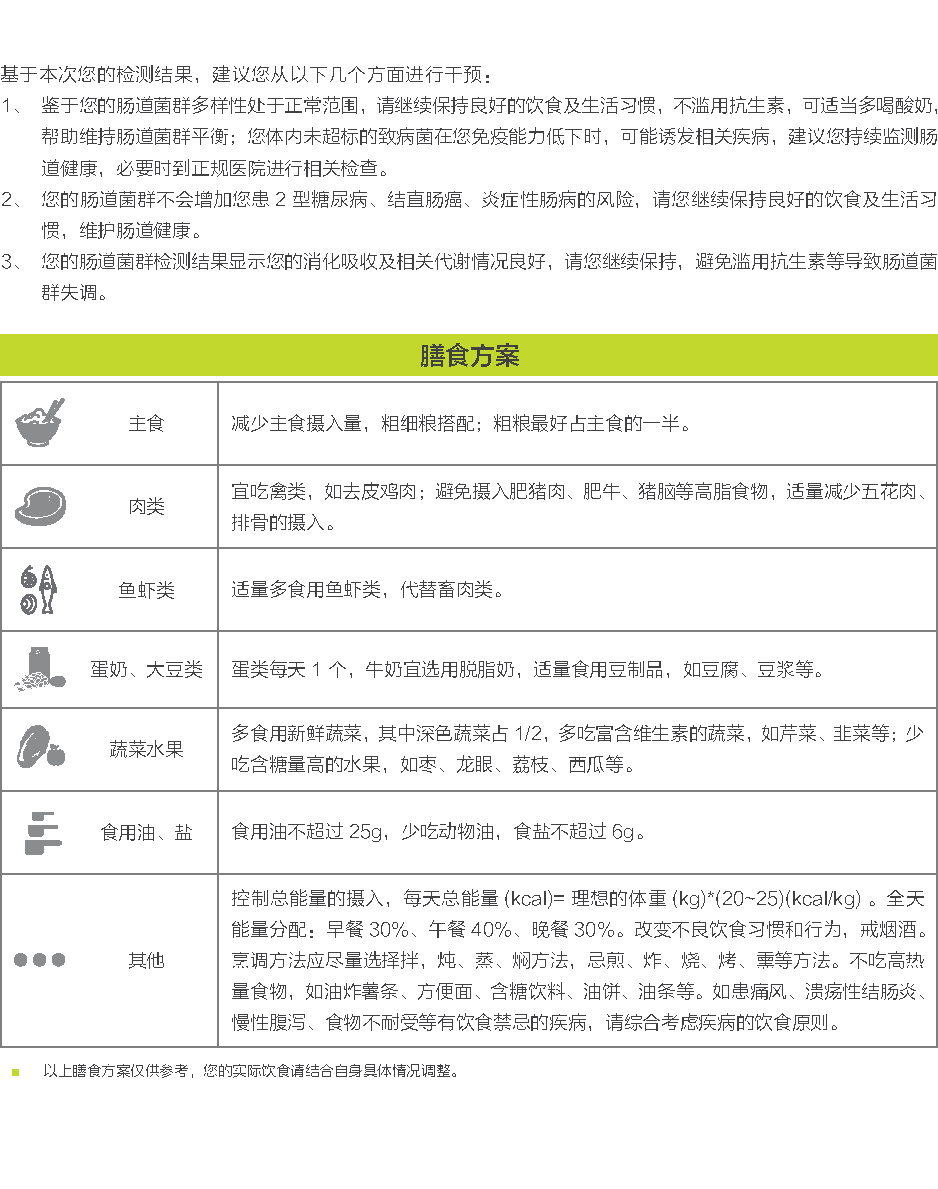
\includegraphics[width=\linewidth]{shanshifangan.pdf}

\end{LRaside}


\begin{LRaside}[.70]{肠道调节方案}
\noindent
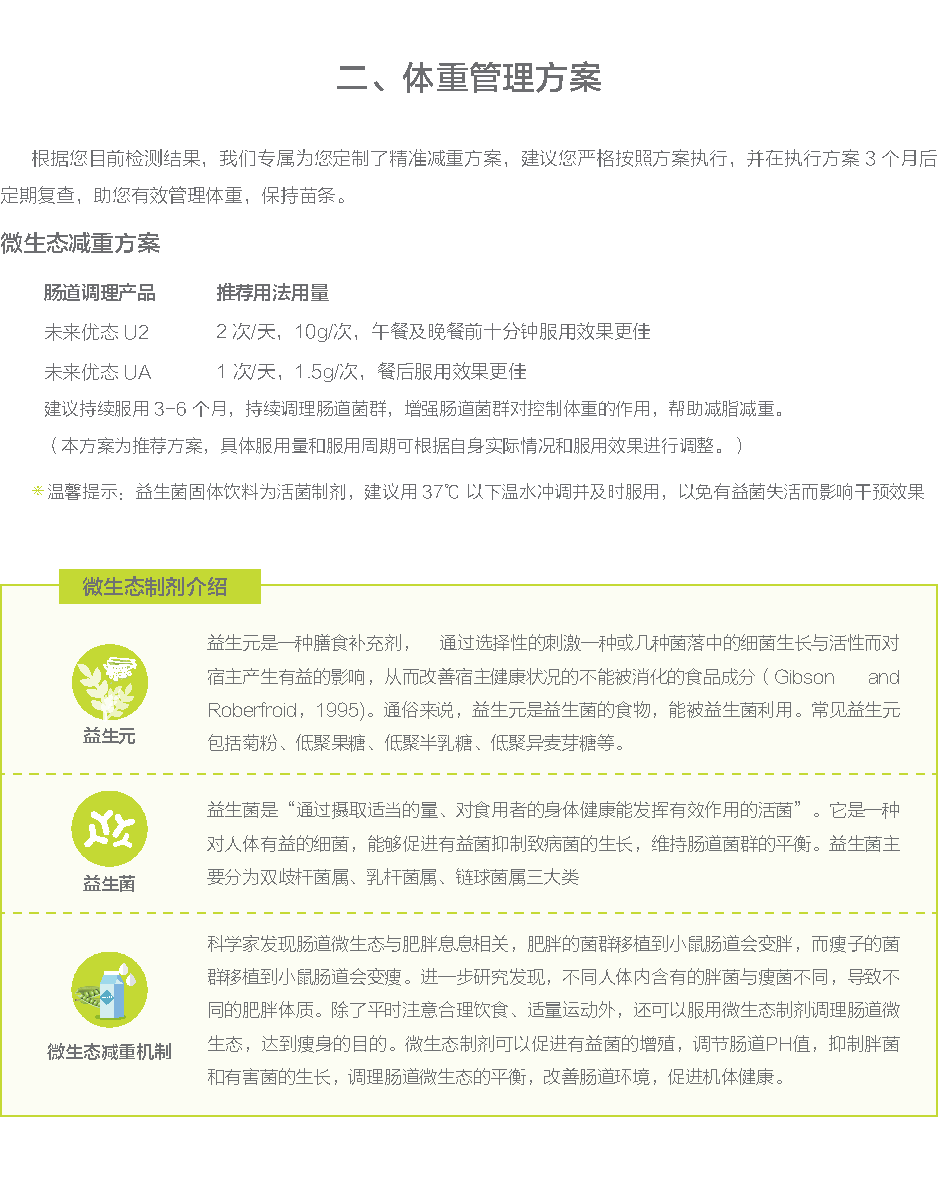
\includegraphics[width=\linewidth]{tiaojiefangan.pdf}

\asidebreak %
{\bf *综合您肠道菌群、营养功能检测结果,为您定制以下肠道调节方案:}\\
{\bf 益生元和益生菌}\\{\indent 1.每天服用适量益生菌产品(如乳双歧杆菌活菌制剂等),增加肠道内益生菌的数量,抑制有害菌的生长。

2.每天可服用适量低聚糖类产品,如低聚果糖、低聚半乳糖、低聚异麦芽糖、低聚甘露糖,促进体内双歧杆菌、乳杆菌等益生菌的生长。 

3.如患炎症性肠病、慢性腹泻,不宜服用菊粉及低聚果糖,建议选择低聚半乳糖。}\\
\end{LRaside}

\begin{LRaside}[.20]{运动方案}
{\bf *适量运动可以帮助改善肠道菌群}\\
建议您:\\
{\indent 养成每天运动的好习惯。尽量减少静坐时间,每小时起来活动2\textasciitilde 3分钟。可根据自己的喜好选择运动方式,如快步走、跑步、球类、爬山、游泳等。也可利用零碎的时间做耐力运动,如哑铃、深蹲、俯卧撑、跳绳、有氧操等。每天运动30分钟以上,每周3-5次。}
\asidebreak %
\noindent

\includegraphics[width=\linewidth]{yundongfangan.pdf}

\end{LRaside}

%{\noindent\qihao *以上健康建议仅供参考,您的实际饮食、保健、运动等还需结合自身具体情况。}

\end{document}
